\documentclass[a4paper, 12pt]{article}
\usepackage[left=1.5cm, right=1.5cm, top=1.5cm, bottom=2.5cm]{geometry}
\usepackage[utf8]{inputenc}
\usepackage[russian]{babel}
\usepackage{verbatim}
\usepackage{graphicx}
\usepackage{listingsutf8}
\usepackage{color}
\usepackage{ulem}
\usepackage{amsmath}
\usepackage{array}
\usepackage{amssymb, latexsym, amsmath, textcomp}
\usepackage{indentfirst}
\usepackage{cmap}
\usepackage{graphics}
\usepackage{listings}
\usepackage{enumerate}
\usepackage{wrapfig}

\lstset{
basicstyle=\footnotesize,
breaklines=true,
numbers=left,
extendedchars=\true,
numbersep=7pt,
caption=\lstname,
frame=single,
inputencoding=utf8,
showstringspaces=\false
}

\newenvironment{enumerate*}%
  {\begin{enumerate}%
    \setlength{\itemsep}{1pt}%
    \setlength{\parskip}{1pt}}%
  {\end{enumerate}}
\newenvironment{itemize*}%
  {\begin{itemize}%
    \setlength{\itemsep}{1pt}%
    \setlength{\parskip}{1pt}}%
  {\end{itemize}}

%------------------------------------------------------------------------------------------------------------------------------
%------------------------------------------------------------------------------------------------------------------------------
\begin{document}

\begin{titlepage}
\begin{center}
{Санкт-Петербургский национальный исследовательский университет информационных технологий, механики и оптики}

Кафедра вычислительной техники
\end{center}
\vspace{50mm}
\begin{center}
\begin{tabular}{c}
\Huge{\textbf{Отчёт}}\\
\Large{\textbf{по лабораторной работе №3}}\\
\Large{\textbf{дисциплины <<Программирование интернет-приложений>>}}\\
\Large{\textbf{Вариант №374}}\\[2mm]
\end{tabular}
\end{center}
\vspace{85mm}
\begin{flushright}
\begin{tabular}{l}
Выполнили:\\
студенты гр. P3211\\
Ефремов Р.В.,\\
Синицкий Д.П.\\
Преподаватели:\\
Цопа Е.А.\\
Письмак А.Е.\\
\\
\end{tabular}
\end{flushright}
\vspace{15mm}
\begin{center}
Санкт-Петербург - 2017 г.
\end{center}
\end{titlepage}
\newpage

\section{Текст задания}


\begin{wrapfigure}{r}{0.4\textwidth}
\begin{center}
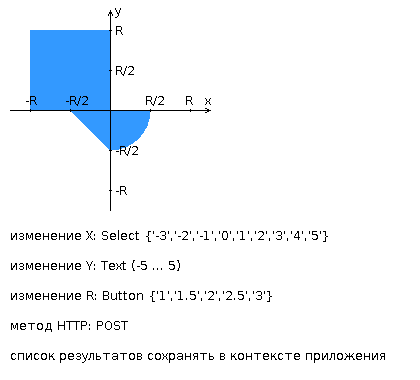
\includegraphics[width=0.4\textwidth]{img/areas.png}
\end{center}
\end{wrapfigure}

Разработать приложение на базе JavaServer Faces Framework, которое осуществляет проверку попадания точки в заданную область на координатной плоскости.

Приложение должно включать в себя 2 facelets-шаблона - стартовую страницу и основную страницу приложения, а также набор управляемых бинов (managed beans), реализующих логику на стороне сервера.

\paragraph{Стартовая страница должна содержать следующие элементы:}

\begin{itemize*}
\item ''Шапку'', содержащую ФИО студента, номер группы и номер варианта.
\item Интерактивные часы, показывающие текущие дату и время, обновляющиеся раз в 5 секунд.
\item Ссылку, позволяющую перейти на основную страницу приложения

\end{itemize*}

\paragraph{Основная страница приложения должна содержать следующие элементы:}
\begin{itemize*}
\item Набор компонентов для задания координат точки и радиуса области в соответствии с вариантом задания. Может потребоваться использование дополнительных библиотек компонентов - ICEfaces (префикс "ace") и PrimeFaces (префикс "p"). Если компонент допускает ввод заведомо некорректных данных (таких, например, как буквы в координатах точки или отрицательный радиус), то приложение должно осуществлять их валидацию.
\item Динамически обновляемую картинку, изображающую область на координатной плоскости в соответствии с номером варианта и точки, координаты которых были заданы пользователем. Клик по картинке должен инициировать сценарий, осуществляющий определение координат новой точки и отправку их на сервер для проверки её попадания в область. Цвет точек должен зависить от факта попадания / непопадания в область. Смена радиуса также должна инициировать перерисовку картинки.
\item Таблицу со списком результатов предыдущих проверок.
\item Ссылку, позволяющую вернуться на стартовую страницу.
\end{itemize*}


\paragraph{Дополнительные требования к приложению:}
\begin{itemize*}
\item Все результаты проверки должны сохраняться в базе данных под управлением СУБД PostgreSQL.
\item Для доступа к БД необходимо использовать ORM Hibernate.
\item Для управления списком результатов должен использоваться Session-scoped Managed Bean.
\item Конфигурация управляемых бинов должна быть задана с помощью параметров в конфигурационном файле.
\item Правила навигации между страницами приложения должны быть заданы в отдельном конфигурационном файле.
\end{itemize*}

\newpage

\section{Код}

%\lstinputlisting[language=Java, caption=AreaCheckServlet.java]{../src/AreaCheckServlet.java}
%\lstinputlisting[language=Java, caption=ControllerServlet.java]{../src/ControllerServlet.java}
%\lstinputlisting[language=Java, caption=Point.java]{../src/point/Point.java}
%\lstinputlisting[language=HTML, caption=index.jsp{../web/content/index.jsp}
%\lstinputlisting[language=Java, caption=canvas\_drawing.js]{../web/content/canvas_drawing.js}
%\lstinputlisting[language=Java, caption=clickpoint.js]{../web/content/clickpoint.js}
%\lstinputlisting[language=XML, caption=web.xml]{../web/WEB-INF/web.xml}

\section{Выводы по работе}
%В ходе подготовки к выполнению данной лабораторной работы были изучены основы создания веб-приложений с использованием сервлетов по схеме MVC, а именно принципы и правила написания HttpServlet'ов, JSP-страниц, их конфигурация в файле web.xml, .

%С использованием полученных знаний в соответствии с заданием было реализовано и развернуто на сервере Glassfish веб-приложение. 

\end{document}
